\documentclass{article}

% content/resources/templates/preamble.tex
\usepackage[margin=0.6in]{geometry}
\author{Milav Dabgar}
\usepackage{amsmath,amssymb,amsthm}
\usepackage{booktabs}
\usepackage{multirow}
\usepackage{xcolor}
\usepackage{tcolorbox}
\tcbuselibrary{breakable,skins}
\usepackage[colorlinks=true,linkcolor=blue]{hyperref}
\usepackage{titlesec}
\usepackage{enumitem}
\usepackage{tikz}
\usepackage{pgfplots}
\usepackage{circuitikz}
\usepackage[version=4]{mhchem}
\usepackage{longtable}
\usepackage{array}
\usepackage{float}
\usepackage{caption}
\usepackage{listings}

\lstset{
  basicstyle=\small\ttfamily,
  breaklines=true,
  breakatwhitespace=false,
  postbreak=\mbox{\textcolor{red}{$\hookrightarrow$}\space},
  float=false,
  numbers=left,
  numberstyle=\tiny\color{gray},
  numbersep=10pt,
  xleftmargin=2em,
  keywordstyle=\color{blue},
  commentstyle=\color{green!60!black},
  stringstyle=\color{purple},
  backgroundcolor=\color{gray!5},
  showstringspaces=false,
  tabsize=2,
  captionpos=b,
  keepspaces=true,
  columns=flexible
}

\pgfplotsset{compat=1.18}
\usetikzlibrary{shapes,arrows,positioning,calc,patterns,decorations.pathmorphing,decorations.markings,arrows.meta}

% Color scheme
\definecolor{headcolor}{RGB}{0,102,204}
\definecolor{keycolor}{RGB}{220,20,60}
\definecolor{solutioncolor}{RGB}{34,139,34}
\definecolor{mnemoniccolor}{RGB}{148,0,211}
\definecolor{codecolor}{RGB}{0,0,100}

% Spacing
\setlength{\parskip}{3pt}
\setlist[itemize]{nosep}
\setlist[enumerate]{nosep}

% Title formatting
\titleformat{\section}{\Large\bfseries\color{headcolor}}{\thesection}{1em}{}
\titleformat{\subsection}{\large\bfseries\color{headcolor}}{\thesubsection}{1em}{}

% Pandoc tightlist compatibility
\providecommand{\tightlist}{%
  \setlength{\itemsep}{0pt}\setlength{\parskip}{0pt}}

% Pandoc longtable compatibility
\newcounter{none}
\def\thenone{}


% content/resources/templates/english-boxes.tex

% Custom environments
\newtcolorbox{solutionbox}{
 breakable,
 enhanced,
 colback=solutioncolor!5!white,
 colframe=solutioncolor!75!black,
 fonttitle=\bfseries,
 title=Solution
}

\newtcolorbox{solutionboxnobreak}{
 colback=solutioncolor!5!white,
 colframe=solutioncolor!75!black,
 fonttitle=\bfseries,
 title=Solution
}

\newtcolorbox{keyformula}{
 breakable,
 enhanced,
 colback=keycolor!5!white,
 colframe=keycolor!75!black,
 fonttitle=\bfseries,
 title=Key Formula
}

\newtcolorbox{mnemonicboxenv}{
 breakable,
 enhanced,
 colback=mnemoniccolor!5!white,
 colframe=mnemoniccolor!75!black,
 fonttitle=\bfseries,
 title=Mnemonic
}

\newcommand{\mnemonicbox}[1]{%
  \begin{mnemonicboxenv}
    #1
  \end{mnemonicboxenv}
}


% Custom commands for GTU solutions
% This file defines semantic commands for consistent formatting

% Question command with automatic formatting
\newcommand{\question}[2]{%
  \section*{Question #1}%
  \textbf{#2}%
}

% OR question variant
\newcommand{\questionor}[2]{%
  \section*{Question #1 OR}%
  \textbf{#2}%
}

% Proper table environment with caption
\newenvironment{answertable}[1]{%
  \begin{table}[htbp]
  \centering
  \caption{#1}
}{%
  \end{table}
}

% Proper figure environment for diagrams
\newenvironment{answerdiagram}[1]{%
  \begin{figure}[htbp]
  \centering
  \caption{#1}
}{%
  \end{figure}
}

% Semantic markup for key terms
\newcommand{\keyword}[1]{\textbf{#1}}
\newcommand{\code}[1]{\texttt{#1}}
\newcommand{\classname}[1]{\texttt{#1}}
\newcommand{\methodname}[1]{\texttt{#1}}

% Proper quotation marks
\newcommand{\mnemonic}[1]{``#1''}


\title{Embedded System \& Microcontroller Application (4351102) - Winter 2023 Solution}
\date{December 4, 2023}

\begin{document}
\maketitle

\questionmarks{1(a)}{3}{Draw TIFR register and write its full name.}

\begin{solutionbox}
\textbf{Full Name}: Timer/Counter Interrupt Flag Register

\textbf{TIFR Register Diagram:}

\begin{answertable}{TIFR Register}
\begin{tabulary}{\linewidth}{|C|C|C|C|C|C|C|C|}
\hline
\textbf{7} & \textbf{6} & \textbf{5} & \textbf{4} & \textbf{3} & \textbf{2} & \textbf{1} & \textbf{0} \\ \hline
OCF2 & TOV2 & ICF1 & OCF1A & OCF1B & TOV1 & OCF0 & TOV0 \\ \hline
\end{tabulary}
\end{answertable}

\keyword{Bit Descriptions:}
\begin{itemize}
    \item \keyword{TOV0}: Timer0 Overflow Flag
    \item \keyword{OCF0}: Timer0 Output Compare Flag
    \item \keyword{TOV1}: Timer1 Overflow Flag
\end{itemize}
\end{solutionbox}

\begin{mnemonicbox}
\mnemonic{Timer Interrupts Flag Register}
\end{mnemonicbox}

\questionmarks{1(b)}{4}{Discuss data memory of ATmega32.}

\begin{solutionbox}
\textbf{Data Memory Organization:}

\begin{answertable}{Data Memory Map}
\begin{tabulary}{\linewidth}{|L|L|L|L|}
\hline
\textbf{Memory Type} & \textbf{Size} & \textbf{Address Range} & \textbf{Purpose} \\ \hline
\keyword{General Purpose Registers} & 32 bytes & 0x00-0x1F & R0-R31 registers \\ \hline
\keyword{I/O Memory} & 64 bytes & 0x20-0x5F & Control registers \\ \hline
\keyword{Internal SRAM} & 2048 bytes & 0x60-0x85F & Variable storage \\ \hline
\end{tabulary}
\end{answertable}

\begin{itemize}
    \item \keyword{General Purpose Registers}: Used for arithmetic operations and temporary storage.
    \item \keyword{I/O Memory}: Contains peripheral control and status registers.
    \item \keyword{Internal SRAM}: Used for stack, variables, and dynamic memory allocation.
\end{itemize}
\end{solutionbox}

\begin{mnemonicbox}
\mnemonic{General I/O SRAM Memory}
\end{mnemonicbox}

\questionmarks{1(c)}{7}{Draw and explain general block diagram of embedded system.}

\begin{solutionbox}
\textbf{General Block Diagram:}

\begin{answerdiagram}{Embedded System Block Diagram}
\begin{tikzpicture}[auto, node distance=2cm]
    \node [gtu block] (proc) {Processor/\\Microcontroller};
    \node [gtu block, left=of proc] (input) {Input Devices};
    \node [gtu block, right=of proc] (output) {Output Devices};
    \node [gtu block, above=of proc] (mem) {Memory};
    \node [gtu block, below=of proc] (comm) {Communication\\Interface};
    \node [gtu block, below left=1.5cm of proc] (power) {Power Supply};
    \node [gtu block, below right=1.5cm of proc] (clock) {Clock Circuit};

    \path [gtu arrow] (input) -- (proc);
    \path [gtu arrow] (proc) -- (output);
    \path [gtu arrow] (proc) edge[bend right] (mem);
    \path [gtu arrow] (mem) edge[bend right] (proc);
    \path [gtu arrow] (proc) -- (comm);
    \path [gtu arrow] (power) -- (proc);
    \path [gtu arrow] (clock) -- (proc);
\end{tikzpicture}
\end{answerdiagram}

\textbf{Component Functions:}

\begin{answertable}{Component Functions}
\begin{tabulary}{\linewidth}{|L|L|}
\hline
\textbf{Component} & \textbf{Function} \\ \hline
\keyword{Processor} & Controls entire system operation \\ \hline
\keyword{Memory} & Stores program and data \\ \hline
\keyword{Input Devices} & Sensors, switches, keyboards \\ \hline
\keyword{Output Devices} & LEDs, displays, motors \\ \hline
\keyword{Communication} & UART, SPI, I2C interfaces \\ \hline
\end{tabulary}
\end{answertable}

\keyword{Characteristics:}
\begin{itemize}
    \item \keyword{Real-time Operation}: System responds to inputs within defined time limits.
    \item \keyword{Dedicated Function}: Designed for specific applications.
    \item \keyword{Resource Constraints}: Limited memory, power, and processing capability.
\end{itemize}
\end{solutionbox}

\begin{mnemonicbox}
\mnemonic{Processor Memory Input Output Communication}
\end{mnemonicbox}

\orquestionmarks{1(c)}{7}{Define real time operating system and explain its characteristics.}

\begin{solutionbox}
\textbf{Definition}: \keyword{Real Time Operating System (RTOS)} is an operating system that guarantees response within specified time constraints for critical tasks.

\textbf{Characteristics:}

\begin{answertable}{RTOS Characteristics}
\begin{tabulary}{\linewidth}{|L|L|}
\hline
\textbf{Characteristic} & \textbf{Description} \\ \hline
\keyword{Deterministic} & Predictable response times \\ \hline
\keyword{Multitasking} & Multiple tasks execution \\ \hline
\keyword{Priority-based} & High priority tasks first \\ \hline
\keyword{Minimal Latency} & Fast interrupt response \\ \hline
\end{tabulary}
\end{answertable}

\keyword{Key Concepts:}
\begin{itemize}
    \item \keyword{Hard Real-time}: Missing deadline causes system failure.
    \item \keyword{Soft Real-time}: Performance degrades if deadline missed.
    \item \keyword{Task Scheduling}: Preemptive priority-based scheduling ensures critical tasks run first.
\end{itemize}
\end{solutionbox}

\begin{mnemonicbox}
\mnemonic{Deterministic Multitasking Priority Minimal}
\end{mnemonicbox}

\questionmarks{2(a)}{3}{Write Criteria for choosing microcontroller for embedded system.}

\begin{solutionbox}
\textbf{Selection Criteria:}

\begin{answertable}{Selection Criteria}
\begin{tabulary}{\linewidth}{|L|L|}
\hline
\textbf{Criteria} & \textbf{Importance} \\ \hline
\keyword{Processing Speed} & Match application requirements \\ \hline
\keyword{Memory Size} & Sufficient ROM/RAM \\ \hline
\keyword{I/O Pins} & Adequate peripheral interfaces \\ \hline
\keyword{Power Consumption} & Battery life consideration \\ \hline
\keyword{Cost} & Budget constraints \\ \hline
\keyword{Development Tools} & Compiler, debugger availability \\ \hline
\end{tabulary}
\end{answertable}
\end{solutionbox}

\begin{mnemonicbox}
\mnemonic{Speed Memory I/O Power Cost Tools}
\end{mnemonicbox}

\questionmarks{2(b)}{4}{Discuss Harvard Architecture in the AVR.}

\begin{solutionbox}
\textbf{Harvard Architecture Features:}

\begin{answertable}{Harvard Architecture}
\begin{tabulary}{\linewidth}{|L|L|}
\hline
\textbf{Feature} & \textbf{Description} \\ \hline
\keyword{Separate Buses} & Program and data have independent buses \\ \hline
\keyword{Simultaneous Access} & Can fetch instruction and access data simultaneously \\ \hline
\keyword{Different Memory Types} & Flash for program, SRAM for data \\ \hline
\end{tabulary}
\end{answertable}

\begin{answerdiagram}{Harvard Architecture}
\begin{tikzpicture}[auto, node distance=2cm]
    \node [gtu block] (cpu) {CPU};
    \node [gtu block, right=of cpu, yshift=1cm] (prog) {Program Bus};
    \node [gtu block, right=of cpu, yshift=-1cm] (data) {Data Bus};
    \node [gtu block, right=of prog] (flash) {Flash Memory};
    \node [gtu block, right=of data] (sram) {SRAM};

    \path [gtu arrow] (cpu) -- (prog);
    \path [gtu arrow] (cpu) -- (data);
    \path [gtu arrow] (prog) -- (flash);
    \path [gtu arrow] (data) -- (sram);
\end{tikzpicture}
\end{answerdiagram}

\begin{itemize}
    \item \keyword{Advantage}: Higher performance due to parallel access.
    \item \keyword{16-bit Instructions}: Most instructions execute in single clock cycle.
\end{itemize}
\end{solutionbox}

\begin{mnemonicbox}
\mnemonic{Separate Simultaneous Different Performance}
\end{mnemonicbox}

\questionmarks{2(c)}{7}{Discuss different ways of connecting clock sources to the AVR.}

\begin{solutionbox}
\textbf{Clock Sources:}

\begin{answertable}{Clock Source Types}
\begin{tabulary}{\linewidth}{|L|L|L|}
\hline
\textbf{Clock Source} & \textbf{Frequency Range} & \textbf{Application} \\ \hline
\keyword{External Crystal} & 1-16 MHz & High accuracy applications \\ \hline
\keyword{External RC} & 1-8 MHz & Cost-effective solution \\ \hline
\keyword{Internal RC} & 1-8 MHz & Default, no external components \\ \hline
\keyword{External Clock} & Up to 16 MHz & Synchronized systems \\ \hline
\end{tabulary}
\end{answertable}

\keyword{Clock Selection via Fuse Bits:}
\begin{itemize}
    \item \keyword{CKSEL3:0}: Bits determine clock source.
    \item \keyword{CKDIV8}: Bit divides clock by 8.
    \item \keyword{SUT1:0}: Bits set startup time.
\end{itemize}

\keyword{Descriptions:}
\begin{itemize}
    \item \keyword{Crystal Oscillator}: Most stable, requires external crystal and capacitors.
    \item \keyword{RC Oscillator}: Less accurate but cheaper.
    \item \keyword{Internal Oscillator}: Factory calibrated, temperature dependent.
\end{itemize}
\end{solutionbox}

\begin{mnemonicbox}
\mnemonic{Crystal RC Internal External}
\end{mnemonicbox}

\orquestionmarks{2(a)}{3}{Write size of code ROM, SRAM and EEPROM, Number of I/O pins, ADC and Timers for ATmega32.}

\begin{solutionbox}
\textbf{ATmega32 Specifications:}

\begin{answertable}{Device Specifications}
\begin{tabulary}{\linewidth}{|L|L|}
\hline
\textbf{Specification} & \textbf{ATmega32} \\ \hline
\keyword{Flash ROM} & 32 KB \\ \hline
\keyword{SRAM} & 2 KB \\ \hline
\keyword{EEPROM} & 1 KB \\ \hline
\keyword{I/O Pins} & 32 pins \\ \hline
\keyword{ADC Channels} & 8 channels \\ \hline
\keyword{Timers} & 3 timers \\ \hline
\end{tabulary}
\end{answertable}
\end{solutionbox}

\begin{mnemonicbox}
\mnemonic{32K Flash 2K SRAM 1K EEPROM 32 I/O 8 ADC 3 Timers}
\end{mnemonicbox}

\orquestionmarks{2(b)}{4}{Draw ATmega32 pin diagram and write function of Vcc, AVcc and Aref pin.}

\begin{solutionbox}
\textbf{ATmega32 Pin Functions:}

\begin{answertable}{Pin Functions}
\begin{tabulary}{\linewidth}{|L|L|}
\hline
\textbf{Pin} & \textbf{Function} \\ \hline
\keyword{Vcc} & Main power supply (+5V) \\ \hline
\keyword{AVcc} & Analog power supply for ADC \\ \hline
\keyword{Aref} & ADC reference voltage \\ \hline
\end{tabulary}
\end{answertable}

\begin{center}
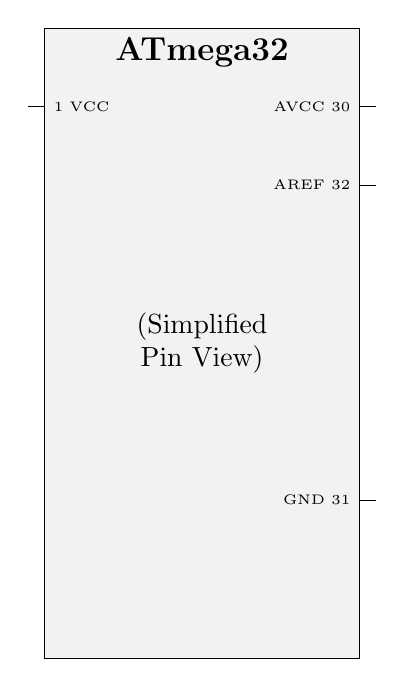
\begin{tikzpicture}[
    pin/.style={draw, rectangle, minimum width=2.5cm, minimum height=0.5cm, font=\small},
    ic/.style={draw, rectangle, minimum width=4cm, minimum height=8cm, fill=gray!10}
]
    \node [ic] (body) {};
    \node [anchor=north, font=\large\bfseries] at (body.north) {ATmega32};

    % Selected Pins for Diagram
    \node [anchor=west, font=\tiny] at ([yshift=-1cm]body.north west) {1 VCC};
    \draw ([yshift=-1cm]body.north west) -- +(-0.2,0);
    
    \node [anchor=east, font=\tiny] at ([yshift=-1cm]body.north east) {AVCC 30};
    \draw ([yshift=-1cm]body.north east) -- +(0.2,0);

    \node [anchor=east, font=\tiny] at ([yshift=-2cm]body.north east) {AREF 32};
    \draw ([yshift=-2cm]body.north east) -- +(0.2,0);

     \node [anchor=east, font=\tiny] at ([yshift=-6cm]body.north east) {GND 31};
    \draw ([yshift=-6cm]body.north east) -- +(0.2,0);
    
    \node [align=center] at (body.center) { (Simplified\\Pin View)};

\end{tikzpicture}
\end{center}

\begin{itemize}
    \item \keyword{Vcc}: Supplies power to digital circuits.
    \item \keyword{AVcc}: Separate supply for ADC to reduce noise.
    \item \keyword{Aref}: External reference for ADC conversion.
\end{itemize}
\end{solutionbox}

\begin{mnemonicbox}
\mnemonic{Vcc Digital AVcc Analog Aref Reference}
\end{mnemonicbox}

\orquestionmarks{2(c)}{7}{Explain AVR status register in detail.}

\begin{solutionbox}
\textbf{SREG (Status Register) Bits:}

\begin{answertable}{SREG Bits}
\begin{tabulary}{\linewidth}{|C|C|L|}
\hline
\textbf{Bit} & \textbf{Name} & \textbf{Function} \\ \hline
7 & I & Global Interrupt Enable \\ \hline
6 & T & Bit Copy Storage \\ \hline
5 & H & Half Carry Flag \\ \hline
4 & S & Sign Flag \\ \hline
3 & V & Overflow Flag \\ \hline
2 & N & Negative Flag \\ \hline
1 & Z & Zero Flag \\ \hline
0 & C & Carry Flag \\ \hline
\end{tabulary}
\end{answertable}

\begin{answertable}{SREG Layout}
\begin{tabulary}{\linewidth}{|C|C|C|C|C|C|C|C|}
\hline
\textbf{I} & \textbf{T} & \textbf{H} & \textbf{S} & \textbf{V} & \textbf{N} & \textbf{Z} & \textbf{C} \\ \hline
7 & 6 & 5 & 4 & 3 & 2 & 1 & 0 \\ \hline
\end{tabulary}
\end{answertable}

\keyword{Bit Details:}
\begin{itemize}
    \item \keyword{I Flag}: Controls global interrupt enable/disable.
    \item \keyword{Arithmetic Flags}: C, Z, N, V, S, H updated after ALU operations.
    \item \keyword{T Flag}: Used by BLD and BST instructions for bit manipulation.
\end{itemize}
\end{solutionbox}

\begin{mnemonicbox}
\mnemonic{I Transfer Half Sign oVerflow Negative Zero Carry}
\end{mnemonicbox}

\questionmarks{3(a)}{3}{Explain RESET circuit for the AVR microcontroller.}

\begin{solutionbox}
\textbf{Reset Sources:}

\begin{answertable}{Reset Sources}
\begin{tabulary}{\linewidth}{|L|L|}
\hline
\textbf{Reset Source} & \textbf{Description} \\ \hline
\keyword{Power-on Reset} & When power is applied \\ \hline
\keyword{External Reset} & Through RESET pin \\ \hline
\keyword{Brown-out Reset} & When voltage drops \\ \hline
\keyword{Watchdog Reset} & Watchdog timer overflow \\ \hline
\end{tabulary}
\end{answertable}

\textbf{Reset Circuit:}

\begin{center}
\begin{tikzpicture}[auto, node distance=1.5cm]
    \node (vcc) {Vcc};
    \node [below=of vcc] (node1) {};
    \node [below=of node1] (gnd) {GND};
    \node [right=of node1] (reset) {RESET Pin};

    \draw (vcc) -- node[left] {R} (node1);
    \draw (node1) -- node[left] {C} (gnd);
    \draw (node1) -- (reset);
\end{tikzpicture}
\end{center}

\begin{itemize}
    \item \keyword{Reset Duration}: Minimum 2 clock cycles.
    \item \keyword{Reset Vector}: Program starts from address 0x0000.
\end{itemize}
\end{solutionbox}

\begin{mnemonicbox}
\mnemonic{Power External Brown-out Watchdog}
\end{mnemonicbox}

\questionmarks{3(b)}{4}{List I/O registers associated with EEPROM. Write programming steps to write data on EEPROM.}

\begin{solutionbox}
\textbf{EEPROM Registers:}

\begin{answertable}{EEPROM Registers}
\begin{tabulary}{\linewidth}{|L|L|}
\hline
\textbf{Register} & \textbf{Function} \\ \hline
\keyword{EEAR} & EEPROM Address Register \\ \hline
\keyword{EEDR} & EEPROM Data Register \\ \hline
\keyword{EECR} & EEPROM Control Register \\ \hline
\end{tabulary}
\end{answertable}

\textbf{Programming Steps:}
\begin{enumerate}
    \item Wait for previous write to complete (check \keyword{EEWE} bit).
    \item Set address in \keyword{EEAR} register.
    \item Set data in \keyword{EEDR} register.
    \item Set \keyword{EEMWE} bit in \keyword{EECR}.
    \item Set \keyword{EEWE} bit within 4 clock cycles.
\end{enumerate}
\end{solutionbox}

\begin{mnemonicbox}
\mnemonic{Wait Address Data Master-Write Enable-Write}
\end{mnemonicbox}

\questionmarks{3(c)}{7}{Draw and explain TCCR0 register in detail.}

\begin{solutionbox}
\textbf{TCCR0 (Timer/Counter0 Control Register):}

\begin{answertable}{TCCR0 Bits}
\begin{tabulary}{\linewidth}{|C|C|L|}
\hline
\textbf{Bit} & \textbf{Name} & \textbf{Function} \\ \hline
7 & FOC0 & Force Output Compare \\ \hline
6,3 & WGM01/00 & Waveform Generation Mode \\ \hline
5,4 & COM01/00 & Compare Output Mode \\ \hline
2,1,0 & CS02/01/00 & Clock Select \\ \hline
\end{tabulary}
\end{answertable}

\begin{answertable}{TCCR0 Layout}
\begin{tabulary}{\linewidth}{|C|C|C|C|C|C|C|C|}
\hline
\textbf{FOC0} & \textbf{WGM01} & \textbf{COM01} & \textbf{COM00} & \textbf{WGM00} & \textbf{CS02} & \textbf{CS01} & \textbf{CS00} \\ \hline
7 & 6 & 5 & 4 & 3 & 2 & 1 & 0 \\ \hline
\end{tabulary}
\end{answertable}

\keyword{Clock Select Options:}
\begin{itemize}
    \item \keyword{000}: No clock (Timer stopped)
    \item \keyword{001}: clk/1 (No prescaling)
    \item \keyword{010}: clk/8, \keyword{011}: clk/64
    \item \keyword{100}: clk/256, \keyword{101}: clk/1024
\end{itemize}
\end{solutionbox}

\begin{mnemonicbox}
\mnemonic{Force Waveform Compare Clock Select}
\end{mnemonicbox}

\orquestionmarks{3(a)}{3}{List registers associated with Timer 1.}

\begin{solutionbox}
\textbf{Timer1 Registers:}

\begin{answertable}{Timer1 Registers}
\begin{tabulary}{\linewidth}{|L|L|}
\hline
\textbf{Register} & \textbf{Function} \\ \hline
\keyword{TCCR1A} & Timer1 Control Register A \\ \hline
\keyword{TCCR1B} & Timer1 Control Register B \\ \hline
\keyword{TCNT1H/L} & Timer1 Counter Register \\ \hline
\keyword{OCR1AH/L} & Output Compare Register A \\ \hline
\keyword{OCR1BH/L} & Output Compare Register B \\ \hline
\keyword{ICR1H/L} & Input Capture Register \\ \hline
\end{tabulary}
\end{answertable}
\end{solutionbox}

\begin{mnemonicbox}
\mnemonic{Control Counter Output-Compare Input-Capture}
\end{mnemonicbox}

\orquestionmarks{3(b)}{4}{Write an AVR C program to store 'G' into location 0x005F of EEPROM.}

\begin{solutionbox}
\textbf{Program:}

\begin{lstlisting}[language=C]
#include <avr/io.h>
#include <avr/eeprom.h>

void eeprom_write_byte_custom(uint16_t addr, uint8_t data)
{
    while(EECR & (1<<EEWE));  // Wait for previous write
    EEAR = addr;              // Set address
    EEDR = data;              // Set data
    EECR |= (1<<EEMWE);       // Master write enable
    EECR |= (1<<EEWE);        // Write enable
}

int main()
{
    eeprom_write_byte_custom(0x005F, 'G');
    return 0;
}
\end{lstlisting}

\keyword{Program Steps:}
\begin{itemize}
    \item Check \keyword{EEWE} bit for completion.
    \item Load address \code{0x005F} into \keyword{EEAR}.
    \item Load 'G' (ASCII 71) into \keyword{EEDR}.
    \item Enable master write, then write enable.
\end{itemize}
\end{solutionbox}

\begin{mnemonicbox}
\mnemonic{Wait Address Data Master Write}
\end{mnemonicbox}

\orquestionmarks{3(c)}{7}{Write a C program to toggle only the PORTB.4 bit continuously every 70 $\mu$s. Use Timer0, Normal mode, and 1:8 prescaler to create the delay. Assume XTAL = 8 MHz.}

\begin{solutionbox}
\textbf{Calculation:}
\begin{itemize}
    \item \keyword{Clock} = 8MHz/8 = 1MHz ($1\mu s$ period).
    \item For $70\mu s$: \keyword{Count} = 70 cycles.
    \item \keyword{Initial value} = $256 - 70 = 186$.
\end{itemize}

\textbf{Program:}

\begin{lstlisting}[language=C]
#include <avr/io.h>

int main()
{
    DDRB |= (1<<4);           // Set PB4 as output
    TCCR0 = 0x02;             // Prescaler 1:8
    
    while(1)
    {
        TCNT0 = 186;          // Load initial value
        while(!(TIFR & (1<<TOV0))); // Wait for overflow
        TIFR |= (1<<TOV0);    // Clear flag
        PORTB ^= (1<<4);      // Toggle PB4
    }
    return 0;
}
\end{lstlisting}
\end{solutionbox}

\begin{mnemonicbox}
\mnemonic{Direction Control Count Wait Clear Toggle}
\end{mnemonicbox}

\questionmarks{4(a)}{3}{Write an AVR C program to monitor bit 5 of port C. If it is HIGH, send 55H to Port B; otherwise, send AAH to Port B.}

\begin{solutionbox}
\textbf{Program:}

\begin{lstlisting}[language=C]
#include <avr/io.h>

int main()
{
    DDRC &= ~(1<<5);          // PC5 as input
    DDRB = 0xFF;              // Port B as output
    
    while(1)
    {
        if(PINC & (1<<5))     // Check PC5
            PORTB = 0x55;     // Send 55H if HIGH
        else
            PORTB = 0xAA;     // Send AAH if LOW
    }
    return 0;
}
\end{lstlisting}

\keyword{Program Logic:}
\begin{itemize}
    \item Configure PC5 as input, Port B as output.
    \item Continuously check PC5 status using bitwise AND.
    \item Output \code{0x55} or \code{0xAA} based on input.
\end{itemize}
\end{solutionbox}

\begin{mnemonicbox}
\mnemonic{Direction Check Output}
\end{mnemonicbox}

\questionmarks{4(b)}{4}{Draw and explain interfacing of LM35 with ATmega32.}

\begin{solutionbox}
\textbf{LM35 Interface:}

\begin{answerdiagram}{LM35 Connection}
\begin{tikzpicture}[auto, node distance=2cm]
    \node [gtu block] (lm35) {LM35\\Sensor};
    \node [gtu block, right=of lm35] (mcu) {ATmega32\\(ADC)};
    
    \draw [gtu arrow] (lm35) -- node[midway, above] {Vout} node[midway, below] {(10mV/$^\circ$C)} (mcu);
    
    \node [above=0.5cm of lm35] (vcc) {+5V};
    \node [below=0.5cm of lm35] (gnd) {GND};
    \draw [gtu arrow] (vcc) -- (lm35);
    \draw [gtu arrow] (lm35) -- (gnd);
    
    \node [right=0.1cm of mcu] (adc) {PA0 (ADC0)};
\end{tikzpicture}
\end{answerdiagram}

\begin{answertable}{Connection Details}
\begin{tabulary}{\linewidth}{|L|L|L|}
\hline
\textbf{LM35 Pin} & \textbf{ATmega32 Pin} & \textbf{Function} \\ \hline
Vcc & +5V & Power supply \\ \hline
Output & PA0 (ADC0) & Analog voltage \\ \hline
GND & GND & Ground \\ \hline
\end{tabulary}
\end{answertable}

\keyword{Specifications:}
\begin{itemize}
    \item \keyword{Temperature Conversion}: 10mV/$^\circ$C output.
    \item \keyword{ADC Resolution}: 10-bit (0-1023).
    \item \keyword{Voltage Range}: 0V to 5V (0$^\circ$C to 500$^\circ$C).
\end{itemize}
\end{solutionbox}

\begin{mnemonicbox}
\mnemonic{Power Output Ground Temperature}
\end{mnemonicbox}

\questionmarks{4(c)}{7}{Draw and explain interfacing of MAX7221 with ATmega32.}

\begin{solutionbox}
\textbf{MAX7221 Interface:}

\begin{answerdiagram}{MAX7221 Connection}
\begin{tikzpicture}[auto, node distance=2cm]
    \node [gtu block] (mcu) {ATmega32};
    \node [gtu block, right=of mcu] (max) {MAX7221};
    \node [gtu block, right=of max] (disp) {7-Segment\\Display};

    \draw [gtu arrow] (mcu.20) -- node[above, font=\tiny] {MOSI (PB5)} (max.160);
    \draw [gtu arrow] (mcu.0) -- node[above, font=\tiny] {SCK (PB7)} (max.180);
    \draw [gtu arrow] (mcu.-20) -- node[above, font=\tiny] {SS (PB4)} (max.200);
    \draw [gtu arrow] (max) -- (disp);
\end{tikzpicture}
\end{answerdiagram}

\begin{answertable}{Pin Connections}
\begin{tabulary}{\linewidth}{|L|L|L|}
\hline
\textbf{MAX7221 Pin} & \textbf{ATmega32 Pin} & \textbf{Function} \\ \hline
DIN & MOSI (PB5) & Serial data input \\ \hline
CLK & SCK (PB7) & Serial clock \\ \hline
LOAD & SS (PB4) & Chip select \\ \hline
\end{tabulary}
\end{answertable}

\keyword{Features:}
\begin{itemize}
    \item \keyword{SPI Interface}: Serial communication protocol.
    \item \keyword{8-Digit Display}: Controls up to 8 common-cathode seven-segment displays.
    \item \keyword{Built-in Decoder}: BCD to seven-segment conversion.
    \item \keyword{Brightness Control}: 16 intensity levels via register.
\end{itemize}

\keyword{Programming Steps:}
\begin{enumerate}
    \item Initialize SPI in master mode.
    \item Send address and data bytes.
    \item Pulse LOAD signal to latch data.
\end{enumerate}
\end{solutionbox}

\begin{mnemonicbox}
\mnemonic{Serial Clock Load Display}
\end{mnemonicbox}

\orquestionmarks{4(a)}{3}{Write an AVR C program to get a byte of data from Port B, and then send it to Port C.}

\begin{solutionbox}
\textbf{Program:}

\begin{lstlisting}[language=C]
#include <avr/io.h>

int main()
{
    DDRB = 0x00;              // Port B as input
    DDRC = 0xFF;              // Port C as output
    
    unsigned char data;
    
    while(1)
    {
        data = PINB;          // Read from Port B
        PORTC = data;         // Send to Port C
    }
    return 0;
}
\end{lstlisting}

\keyword{Program Function:}
\begin{itemize}
    \item Configure Port B as input, Port C as output.
    \item Continuously read from \keyword{PINB} and write to \keyword{PORTC}.
\end{itemize}
\end{solutionbox}

\begin{mnemonicbox}
\mnemonic{Input Output Read Write}
\end{mnemonicbox}

\orquestionmarks{4(b)}{4}{Draw and explain interfacing of ULN2803 with ATmega32.}

\begin{solutionbox}
\textbf{ULN2803 Interface:}

\begin{answerdiagram}{ULN2803 Connection}
\begin{tikzpicture}[auto, node distance=2cm]
    \node [gtu block] (mcu) {ATmega32\\Port};
    \node [gtu block, right=of mcu] (uln) {ULN2803};
    \node [gtu block, right=of uln] (load) {Load/Relay};
    \node [above=0.5cm of load] (vcc) {Vcc};

    \draw [gtu arrow] (mcu) -- node[midway, above, font=\tiny] {Input} (uln);
    \draw [gtu arrow] (uln) -- node[midway, above, font=\tiny] {Output} (load);
    \draw [gtu arrow] (vcc) -- (load);
\end{tikzpicture}
\end{answerdiagram}

\keyword{ULN2803 Features:}
\begin{itemize}
    \item \keyword{8 Darlington Arrays}: High current switching.
    \item \keyword{Input Current}: 500$\mu$A typical.
    \item \keyword{Output Current}: 500mA per channel.
    \item \keyword{Built-in Flyback Diodes}: Inductive load protection.
\end{itemize}

\keyword{Operation}:
\begin{itemize}
    \item \keyword{Application}: Drive relays, motors, solenoids.
    \item \keyword{Active Low Output}: Output goes low (sinks current) when input is high.
\end{itemize}
\end{solutionbox}

\begin{mnemonicbox}
\mnemonic{Darlington Current Protection Drive}
\end{mnemonicbox}

\orquestionmarks{4(c)}{7}{Discuss registers used to program SPI in the AVR.}

\begin{solutionbox}
\textbf{SPI Registers:}

\begin{answertable}{SPI Register Summary}
\begin{tabulary}{\linewidth}{|L|L|L|}
\hline
\textbf{Register} & \textbf{Bits} & \textbf{Function} \\ \hline
\keyword{SPCR} & SPE, DORD, MSTR, CPOL & SPI Control Register \\ \hline
\keyword{SPSR} & SPIF, WCOL, SPI2X & SPI Status Register \\ \hline
\keyword{SPDR} & - & SPI Data Register \\ \hline
\end{tabulary}
\end{answertable}

\keyword{SPCR Register Bits:}
\begin{itemize}
    \item \keyword{SPE}: SPI Enable.
    \item \keyword{DORD}: Data Order (MSB/LSB first).
    \item \keyword{MSTR}: Master/Slave Select.
    \item \keyword{CPOL}: Clock Polarity.
    \item \keyword{CPHA}: Clock Phase.
\end{itemize}

\keyword{SPSR Register Bits:}
\begin{itemize}
    \item \keyword{SPIF}: SPI Interrupt Flag.
    \item \keyword{WCOL}: Write Collision Flag.
    \item \keyword{SPI2X}: Double Speed Mode.
\end{itemize}

\keyword{Programming Sequence:}
\begin{enumerate}
    \item Configure SPI pins as input/output.
    \item Set SPCR register for desired mode.
    \item Write data to SPDR.
    \item Wait for SPIF flag.
    \item Read received data from SPDR.
\end{enumerate}
\end{solutionbox}

\begin{mnemonicbox}
\mnemonic{Control Status Data Enable Order Master}
\end{mnemonicbox}

\questionmarks{5(a)}{3}{Draw and explain pin diagram of L293D motor driver IC.}

\begin{solutionbox}
\textbf{L293D Pinout:}

\begin{center}
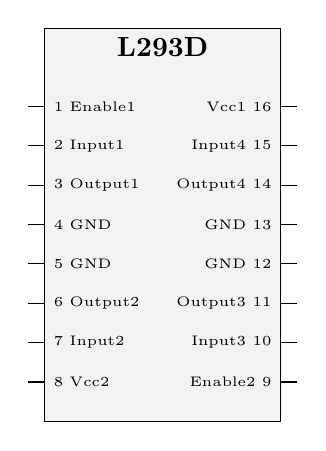
\begin{tikzpicture}[
    pin/.style={draw, rectangle, minimum width=2cm, minimum height=0.5cm, font=\tiny},
    ic/.style={draw, rectangle, minimum width=3cm, minimum height=5cm, fill=gray!10}
]
    \node [ic] (body) {};
    \node [anchor=north, font=\bfseries] at (body.north) {L293D};

    % Pins Left
    \foreach \i/\label in {1/Enable1, 2/Input1, 3/Output1, 4/GND, 5/GND, 6/Output2, 7/Input2, 8/Vcc2} {
        \node [anchor=west, font=\tiny] at ([yshift=-0.5cm-\i*0.5cm]body.north west) {\i\ \label};
        \draw ([yshift=-0.5cm-\i*0.5cm]body.north west) -- +(-0.2,0);
    }

    % Pins Right
    \foreach \i/\label in {16/Vcc1, 15/Input4, 14/Output4, 13/GND, 12/GND, 11/Output3, 10/Input3, 9/Enable2} {
        \pgfmathsetmacro{\ypos}{17-\i}
        \node [anchor=east, font=\tiny] at ([yshift=-0.5cm-\ypos*0.5cm]body.north east) {\label\ \i};
        \draw ([yshift=-0.5cm-\ypos*0.5cm]body.north east) -- +(0.2,0);
    }
\end{tikzpicture}
\end{center}

\keyword{Pin Functions:}
\begin{itemize}
    \item \keyword{1A, 2A}: Input signals for Motor 1.
    \item \keyword{1Y, 2Y}: Output to Motor 1.
    \item \keyword{1EN, 2EN}: Enable pins for motors.
    \item \keyword{Vcc1}: Logic supply (+5V).
    \item \keyword{Vcc2}: Motor supply (+12V).
\end{itemize}
\end{solutionbox}

\begin{mnemonicbox}
\mnemonic{Input Output Enable Logic Motor Supply}
\end{mnemonicbox}

\questionmarks{5(b)}{4}{Draw and explain ADMUX register.}

\begin{solutionbox}
\textbf{ADMUX (ADC Multiplexer Selection Register):}

\begin{answertable}{ADMUX Register}
\begin{tabulary}{\linewidth}{|C|C|L|}
\hline
\textbf{Bit} & \textbf{Name} & \textbf{Function} \\ \hline
7,6 & REFS1/0 & Reference Selection \\ \hline
5 & ADLAR & ADC Left Adjust Result \\ \hline
4-0 & MUX4-0 & Analog Channel Selection \\ \hline
\end{tabulary}
\end{answertable}

\begin{answertable}{ADMUX Bits}
\begin{tabulary}{\linewidth}{|C|C|C|C|C|C|C|C|}
\hline
\textbf{REFS1} & \textbf{REFS0} & \textbf{ADLAR} & \textbf{MUX4} & \textbf{MUX3} & \textbf{MUX2} & \textbf{MUX1} & \textbf{MUX0} \\ \hline
7 & 6 & 5 & 4 & 3 & 2 & 1 & 0 \\ \hline
\end{tabulary}
\end{answertable}

\keyword{Reference Selection (REFS1:0):}
\begin{itemize}
    \item \keyword{00}: AREF pin.
    \item \keyword{01}: AVcc with external capacitor.
    \item \keyword{11}: Internal 2.56V reference.
\end{itemize}

\keyword{Channel Selection}: MUX bits select ADC0-ADC7 channels.
\end{solutionbox}

\begin{mnemonicbox}
\mnemonic{Reference Adjust Multiplexer Channel}
\end{mnemonicbox}

\questionmarks{5(c)}{7}{Explain GSM based security system.}

\begin{solutionbox}
\textbf{GSM Security System:}

\begin{answerdiagram}{GSM Security Block Diagram}
\begin{tikzpicture}[auto, node distance=2cm]
    \node [gtu block] (mcu) {Microcontroller};
    \node [gtu block, left=of mcu] (sensor) {Sensors};
    \node [gtu block, right=of mcu] (gsm) {GSM Module};
    \node [gtu block, right=of gsm] (network) {Network};
    \node [gtu block, below=of network] (mobile) {User Mobile};
    \node [gtu block, above=of mcu] (lcd) {Display};
    \node [gtu block, below=of mcu] (keypad) {Keypad};

    \draw [gtu arrow] (sensor) -- (mcu);
    \draw [gtu arrow] (mcu) -- (gsm);
    \draw [gtu arrow] (gsm) -- (network);
    \draw [gtu arrow] (network) -- (mobile);
    \draw [gtu arrow] (keypad) -- (mcu);
    \draw [gtu arrow] (mcu) -- (lcd);
\end{tikzpicture}
\end{answerdiagram}

\textbf{System Components:}
\begin{itemize}
    \item \keyword{Sensors}: PIR (motion), Door (entry) detection.
    \item \keyword{GSM Module}: SMS/Call communication.
    \item \keyword{Microcontroller}: System control and processing.
    \item \keyword{Keypad/Display}: User interface for status and control.
\end{itemize}

\textbf{Working Principle:}
\begin{enumerate}
    \item Sensors detect intrusion.
    \item Microcontroller processes signal.
    \item GSM module sends SMS alert ("Intruder Detected").
    \item User receives notification and can respond remotely.
\end{enumerate}

\textbf{Features:} Remote monitoring, multiple sensors, automatic alerts.
\end{solutionbox}

\begin{mnemonicbox}
\mnemonic{Sensors Process Communicate Alert Control}
\end{mnemonicbox}

\orquestionmarks{5(a)}{3}{Draw circuit diagram to interface DC motor with ATmega32 using L293D motor driver.}

\begin{solutionbox}
\textbf{DC Motor Interface:}

\begin{answerdiagram}{L293D DC Motor Interface}
\begin{tikzpicture}[auto, node distance=2cm]
    \node [gtu block] (mcu) {ATmega32};
    \node [gtu block, right=of mcu] (l293) {L293D};
    \node [gtu block, right=of l293] (motor) {DC Motor};

    \draw [gtu arrow] (mcu.20) -- node[above, font=\tiny] {PA0 (1A)} (l293.160);
    \draw [gtu arrow] (mcu.0) -- node[above, font=\tiny] {PA1 (2A)} (l293.180);
    \draw [gtu arrow] (mcu.-20) -- node[above, font=\tiny] {PA2 (1EN)} (l293.200);

    \draw [gtu arrow] (l293.20) -- node[above, font=\tiny] {1Y} (motor.160);
    \draw [gtu arrow] (l293.-20) -- node[above, font=\tiny] {2Y} (motor.200);

    \node [above=0.5cm of l293] (vcc) {Vcc};
    \draw [gtu arrow] (vcc) -- (l293);
\end{tikzpicture}
\end{answerdiagram}

\keyword{Connection Details:}
\begin{itemize}
    \item \keyword{PA0} to Input 1A.
    \item \keyword{PA1} to Input 2A.
    \item \keyword{PA2} to Enable 1EN.
\end{itemize}

\keyword{Control Logic:}
\begin{itemize}
    \item \keyword{Clockwise}: PA0=1, PA1=0.
    \item \keyword{Counter-Clockwise}: PA0=0, PA1=1.
    \item \keyword{Stop}: PA2=0.
\end{itemize}
\end{solutionbox}

\begin{mnemonicbox}
\mnemonic{Direction Enable Control Stop}
\end{mnemonicbox}

\orquestionmarks{5(b)}{4}{Draw and explain ADCSRA register.}

\begin{solutionbox}
\textbf{ADCSRA (ADC Control and Status Register A):}

\begin{answertable}{ADCSRA Register}
\begin{tabulary}{\linewidth}{|C|C|L|}
\hline
\textbf{Bit} & \textbf{Name} & \textbf{Function} \\ \hline
7 & ADEN & ADC Enable \\ \hline
6 & ADSC & ADC Start Conversion \\ \hline
5 & ADATE & ADC Auto Trigger Enable \\ \hline
4 & ADIF & ADC Interrupt Flag \\ \hline
3 & ADIE & ADC Interrupt Enable \\ \hline
2-0 & ADPS2-0 & ADC Prescaler Select \\ \hline
\end{tabulary}
\end{answertable}

\begin{answertable}{ADCSRA Layout}
\begin{tabulary}{\linewidth}{|C|C|C|C|C|C|C|C|}
\hline
\textbf{ADEN} & \textbf{ADSC} & \textbf{ADATE} & \textbf{ADIF} & \textbf{ADIE} & \textbf{ADPS2} & \textbf{ADPS1} & \textbf{ADPS0} \\ \hline
7 & 6 & 5 & 4 & 3 & 2 & 1 & 0 \\ \hline
\end{tabulary}
\end{answertable}

\keyword{Prescaler Selection:}
\begin{itemize}
    \item \keyword{000, 001}: Division factor 2.
    \item \keyword{010}: Division factor 4.
    \item \keyword{011}: Division factor 8.
\end{itemize}

\keyword{ADC Operation:}
\begin{enumerate}
    \item Set \keyword{ADEN} to enable ADC.
    \item Set \keyword{ADSC} to start conversion.
    \item Wait for \keyword{ADIF} flag.
    \item Read result from \keyword{ADCH:ADCL}.
\end{enumerate}
\end{solutionbox}

\begin{mnemonicbox}
\mnemonic{Enable Start Auto Interrupt Prescaler}
\end{mnemonicbox}

\orquestionmarks{5(c)}{7}{Explain Weather monitoring system.}

\begin{solutionbox}
\textbf{Weather Monitoring System:}

\begin{answerdiagram}{Weather Monitoring Block Diagram}
\begin{tikzpicture}[auto, node distance=2cm]
    \node [gtu block] (mcu) {Microcontroller};
    \node [gtu block, left=of mcu, yshift=1.5cm] (temp) {Temperature\\Sensor};
    \node [gtu block, left=of mcu, yshift=0.5cm] (hum) {Humidity\\Sensor};
    \node [gtu block, left=of mcu, yshift=-0.5cm] (pres) {Pressure\\Sensor};
    \node [gtu block, left=of mcu, yshift=-1.5cm] (rain) {Rain\\Sensor};
    
    \node [gtu block, right=of mcu, yshift=1cm] (disp) {Display};
    \node [gtu block, right=of mcu, yshift=0cm] (log) {Data Logger};
    \node [gtu block, right=of mcu, yshift=-1cm] (wireless) {Wireless\\Module};
    \node [gtu block, right=of wireless] (remote) {Remote\\Monitor};

    \draw [gtu arrow] (temp) -- (mcu);
    \draw [gtu arrow] (hum) -- (mcu);
    \draw [gtu arrow] (pres) -- (mcu);
    \draw [gtu arrow] (rain) -- (mcu);
    
    \draw [gtu arrow] (mcu) -- (disp);
    \draw [gtu arrow] (mcu) -- (log);
    \draw [gtu arrow] (mcu) -- (wireless);
    \draw [gtu arrow] (wireless) -- (remote);
\end{tikzpicture}
\end{answerdiagram}

\textbf{System Components:}
\begin{answertable}{Sensor Components}
\begin{tabulary}{\linewidth}{|L|L|L|}
\hline
\textbf{Sensor} & \textbf{Parameter} & \textbf{Interface} \\ \hline
\keyword{LM35} & Temperature & Analog (ADC) \\ \hline
\keyword{DHT11} & Humidity & Digital \\ \hline
\keyword{BMP180} & Pressure & I2C \\ \hline
\keyword{Rain Sensor} & Precipitation & Digital \\ \hline
\end{tabulary}
\end{answertable}

\keyword{Features:}
\begin{itemize}
    \item \keyword{Multi-parameter Monitoring}: Temperature, humidity, pressure, rainfall.
    \item \keyword{Data Logging}: Store readings in EEPROM/SD card.
    \item \keyword{Real-time Display}: LCD shows current readings.
    \item \keyword{Wireless Communication}: WiFi/GSM for remote monitoring.
    \item \keyword{Alert System}: Threshold-based warnings.
\end{itemize}

\keyword{Applications:}
\begin{itemize}
    \item Agricultural monitoring
    \item Weather forecasting
    \item Environmental research
    \item Smart home automation
\end{itemize}

\keyword{System Benefits:}
\begin{itemize}
    \item \keyword{Automated Data Collection}: Continuous monitoring.
    \item \keyword{Remote Access}: View data from anywhere.
    \item \keyword{Historical Analysis}: Trend identification.
    \item \keyword{Early Warning}: Extreme weather alerts.
\end{itemize}
\end{solutionbox}

\begin{mnemonicbox}
\mnemonic{Temperature Humidity Pressure Rain Display Log Wireless}
\end{mnemonicbox}

\end{document}
